%%==================================================
%% chapter01.tex for BIT Master Thesis
%% modified by yang yating
%% version: 0.1
%% last update: Dec 25th, 2016
%%==================================================
% \chapter{多角度实体类型过度依赖缓解的事件要素抽取模型}
\chapter{基于多角度对比学习的实体类型过度依赖消解}
\label{chap:chapter4}

事件要素抽取任务是事件抽取的关键组成部分,成为了限制事件抽取整体性能的瓶颈。正如章节\ref{section2_2}所述,现有事件要素抽取的建模存在两种不同的定义,其不同定义的一个显著区别为是否将实体提及识别与事件抽取进行分隔,本章节研究在已经给定实体提及的情况下进行的事件要素抽取。

基于给定的实体提及,大多数事件要素模型在建模过程中利用了其正面信息增益,而忽视了实体类型和要素类型间的强关联对性能产生的负面影响。为了更好地研究该负面影响,本章节首先定义实体类型过度依赖并通过实验验证其降低了多种事件要素抽取模型的整体性能。进一步,本章提出了一种基于多角度对比学习的实体类型过度依赖消解方法解决该问题。实验评估表明,提出的方法可以通用有效地消解不同事件要素抽取模型对于实体类型信息的过度依赖。


\section{引言}

作为基于实体的抽取任务,事件要素抽取~\cite{chen2015event,wang2019hmeae,xiangyu2021capturing}主要研究在给定上下文语义信息的情况下如何更好地建模实体提及和事件触发词间的复杂交互。进一步,结合现有的事件要素抽取方法和以ACE2005为代表的事件要素抽取数据集,可以观察到以下两个数据特征:(1)实体类型为事件要素抽取的实体提及提供了主要信息来源。具体地,按照Peng等人~\cite{peng2020learning}在关系抽取任务中的类似设置,将ACE2005数据集中的实体提及替换成对应的实体类型,并以此训练一个事件要素抽取任务的代表性模型DMBERT~\cite{wang2019adversarial}。实验结果表明DMBERT取得了和替换前几乎相同的性能结果。(2)大多数实体类型在事件中仅以少数特定要素类型参与~\cite{hong2011using}。例如,ACE2005数据集中出现了43种实体类型,但有超过74\%的实体类型以少于5种的要素类型参与到事件中。

基于上述两个数据特征,可以得知实体类型信息对于事件要素抽取任务是至关重要的,且与要素类型密切相关。现有事件要素抽取方法基于实体类型信息的重要性,更多地关注其正面信息增益,而忽略了实体类型和要素类型间的相关性带来的潜在负面影响。如表\ref{example_eto}所示,给定目标抽取文本“A rocket holding the first of \underline{two Mars rovers} blasted off Tuesday on a seven-month \underline{voyage} to the planet.”和$Transport$(运输)事件的事件触发词“voyage”,一个性能优良的事件要素抽取模型需要识别出实体类型为$Landing$的实体提及“two Mars rovers”没有以任何要素类型参与到该事件中,即对应的事件要素类型为空。然而,由于其他实体类型为$Landing$的实体提及在训练数据中较高频率地以要素类型$Vehicle$出现在事件中,正如表\ref{example_eto}中所示的句1和句2,使得现有事件要素抽取模型容易受到实体类型$Landing$的误导,将实体提及“two Mars rovers”的要素类型错误地预测为$Vehicle$。

\begin{table}[htp]
\small
\centering
\caption{实体类型过度依赖示例}
\begin{tabular}{l|ccc}
\toprule
\multicolumn{1}{c|}{实例} & \multicolumn{1}{c}{实体类型} & \multicolumn{1}{c}{要素类型标签} & 要素类型预测 \\ \midrule
\begin{tabular}[c]{@{}l@{}}\textbf{例}: A rocket holding the first of \textcolor{blue}{two Mars} \\ \textcolor{blue}{rovers} blasted off Tuesday on a seven-month \\ \textcolor{red}{voyage} to the planet.\end{tabular}            & \multicolumn{1}{c}{Landing}     & \multicolumn{1}{c}{None}             & Vehicle $\times$            \\ \midrule
\begin{tabular}[c]{@{}l@{}}\textbf{句1}: \textcolor{blue}{The rovers'} \textcolor{red}{landing} sites, on opposite \\ sides of the planet, were chosen for their \\ likelihood of holding evidence of water.\end{tabular} & \multicolumn{1}{c}{Landing}     & \multicolumn{1}{c}{Vehicle}          & Vehicle $\checkmark$            \\ \midrule
\begin{tabular}[c]{@{}l@{}}\textbf{句2}: \textcolor{blue}{The bus} was ripped to shreds while \\ \textcolor{red}{traveling} between a residential area and \\ Haifa university.\end{tabular}                             & \multicolumn{1}{c}{Landing}     & \multicolumn{1}{c}{Vehicle}          & Vehicle $\checkmark$             \\ \bottomrule
\end{tabular}
\label{example_eto}
\end{table}

为此,本章首先定义了实体类型过度依赖并通过预实验评估证明了不同事件要素抽取基线模型均受到实体类型过度依赖问题的影响,使得整体性能出现下降。由于实体类型过度依赖是由建模时对实体类型信息的严重依赖导致的,消解该问题可以考虑提升模型学习除实体类型外的更多语义信息的能力。

广泛应用于计算机视觉~\cite{chen2020simple,he2020momentum}和自然语言处理~\cite{fang2020cert,wang2021cline}的对比学习技术是解决这一问题的有效方法,尤其是监督对比学习技术~\cite{khosla2020supervised,liu2021explicit,yang2022supervised},其可将属于同一类型实例(称之为正样本)的特征表示距离拉近,属于不同类型实例(称之为负样本)的特征表示距离推远。然而,在事件要素抽取任务中,直接应用传统的监督对比学习技术只能根据要素类型信息进行特征学习,而无法同时考虑到实体类型信息。

为了解决上述提到的挑战,本章提出基于多角度对比学习的实体类型过度依赖消解方法。在不同的事件要素抽取模型的基础上,提出了通用的多角度实体类型过度依赖消解(Multi-view Entity Type Overdependency Reduction,METOR)模型,其中多角度指正样本角度和负样本角度。基于正样本角度,本章提出了一种加权-选择的对比学习方法,以提升具有相同要素类型但具有不同实体类型的实例特征表示间的相似性。基于负样本角度,本章提出了一种伪正对比学习方法来降低具有不同要素类型但具有相同实体类型的实例特征表示间的相似性。此外,为了提升上述两种对比学习方法间的协作能力,在模型训练过程中提出了一种高效的循环训练策略。本章的主要贡献概括如下:

\begin{itemize}
\item 定义了实体类型过度依赖问题并通过预实验验证了不同事件要素抽取基线模型均受到该问题的影响而导致整体性能下降。
\item 针对实体类型过度依赖问题,本章提出了基于多角度对比学习的实体类型过度依赖消解方法。该方法可以应用于不同基线模型中,由两种对比学习方法和一种循环训练策略组成,其中循环训练策略能够提升不同对比学习方法间的训练协作。
\item 在广泛使用的ACE2005数据集上进行了大量实验。实验结果表明,本章提出的方法能够通用有效地消解不同基线模型的实体类型过度依赖问题,并基于预训练架构取得当前最优性能。
\end{itemize}

\section{实体类型过度依赖定义与验证}
\label{two}
% 启发于Peng等人~\cite{peng2020learning}在关系抽取任务中的实验结果,为了更好地研究实体类型是否为事件要素抽取任务提供了主要的实体提及信息,本节首先遵循其在关系抽取中的相同设置,在ACE 2005英文数据集中使用实体类型替换实体提及并在该设置下训练事件要素模型DMBERT。实验结果表明DMBERT在F1性能指标上相比于替换前仅下降了1\%,验证了实体类型在事件要素抽取任务中为实体提及提供了主要信息。此外,我们还观察到ACE 2005英文数据集中存在43种实体类型,其中32种实体类型参与的角色类型少于5种。此外,当我们只考虑实体-角色类型共现频率大于10的实体类型时,参与少于5个角色类型的实体类型的数量将增加到38个。
如上一章节所述,实体类型为事件要素抽取任务提供了关键信息且和要素类型信息强关联。为了更好地研究实体类型和要素类型之间的关联性,本节首先形式化地定义实体类型过度依赖,并通过预实验评估其对于事件要素抽取性能的影响。

\subsection{定义}

一般来说,事件要素抽取模型由两个主要部分组成:编码器和分类器。其中编码器将实例编码成特征表示,而分类器识别实例的特征表示和不同要素类型的表示间的相似性。由于实体类型构成了实体提及的主要信息,则以实体提及为重要组成部分的特征编码表示依赖于实体类型。假设$G(r_{k})$是由要素类型为$r_{k}$的实例构成的群组,$C(e_{i}, r_{k})$是由实体类型为$e_{i}$和要素类型为$r_{k}$的实例构成的簇,而$\boldsymbol{h}_{ r_{k}}^{M}$和 $\boldsymbol{h}_{e_{i}, r_{k}}^{M}$分别是$G(r_{k})$和$C(e_{i}, r_{k})$由给定事件要素抽取模型$M$的编码器编码得到的表示,则簇级别的实体类型依赖定义如下:
\begin{definition}[实体类型依赖]
\label{definition1}
给定$C(e_{i}, r_{k})$和由$M$编码得到的对应编码表示 $\boldsymbol{h}_{e_{i}, r_{k}}^{M}$,如果存在$C(e_{i}, r_{l})$和$C(e_{j}, r_{k})$ $(i \neq j,\ l \neq k)$满足如下条件,则称
$C(e_{i}, r_{k})$依赖于实体类型$e_{i}$: 
\begin{equation}
\label{equation1}
  \boldsymbol{h}_{e_{i},r_{k}}^{M} \cdot \boldsymbol{h}_{e_{i},r_{l}}^{M} > \boldsymbol{h}_{e_{i},r_{k}}^{M} \cdot \boldsymbol{h}_{e_{j},r_{k}}^{M} 
\end{equation}
\end{definition}
在定义\ref{definition1}中,如果$C(e_{i}, r_{k})$和$C(e_{i}, r_{l})$之间的相似性比$C(e_{i}, r_{k})$和$C(e_{j}, r_{k})$之间的相似性高,则认定$C(e_{i}, r_{k})$满足实体类型依赖定义。该定义阐述了由于实体类型$e_{i}$和要素类型$r_{k}$的关联性使得$C(e_{i}, r_{k})$与群组$G_{r_{l}}$中的$C(e_{i}, r_{l})$的特征表示间的相似性反而比其与同在一个群组中的$C(e_{j}, r_{k})$的特征表示间的相似性更高的现象。

为了进一步评估这种实体类型依赖是否影响事件要素抽取模型的性能,需要定义簇之间的语义不一致性。Ohashi等人~\cite{ohashi2020text}研究发现如果实例特征表示的相似性与其类别标签不一致,则相应的分类器更加容易出现预测错误。因此,簇级别的语义不一致性可以定义如下:
\begin{definition}[语义不一致]
\label{definition2}
给定$C(e_{i}, r_{k})$和由$M$编码得到的对应编码表示$\boldsymbol{h}_{e_{i}, r_{k}}^{M}$,如果存在$G(r_{l})\ (l \neq k) $满足如下条件,则称$C(e_{i}, r_{k})$存在语义不一致:
\begin{equation}
\label{equation2}
     \boldsymbol{h}_{e_{i},r_{k}}^{M} \cdot  \boldsymbol{h}_{r_{l}}^{M} > \boldsymbol{h}_{e_{i},r_{k}}^{M} \cdot \boldsymbol{h}_{r_{k}}^{M} \\
\end{equation}
\end{definition}
% \noindent 其中$\boldsymbol{h}_{r_{l}}^{M}$和 $\boldsymbol{h}_{r_{k}}^{M}$分别是$G(r_{l})$和$G(r_{k})$由事件要素抽取模型$M$的编码器编码得到的表示。

在定义\ref{definition2}中,虽然$C(e_{i}, r_{k})$中实例的要素类型是$r_{k}$而不是$r_{l}$,但$C(e_{i}, r_{k})$与群组$G(r_{k})$的特征表示间的相似性比其与群组$G(r_{l})$的特征表示间的相似性低。然而,理想情况下$C(e_{i}, r_{k})$应该与自身所属的群组相似性更高,否则将出现语义不一致现象,从而使得编码器$M$对应的分类器更容易预测出错。因此,语义不一致性可用于确定存在实体类型依赖的簇是否影响事件要素抽取模型的性能。基于此,定义簇级别的实体类型过度依赖如下:
\begin{definition}[实体类型过度依赖]
\label{definition3}
给定$C(e_{i}, r_{k})$和由$M$编码得到的对应编码表示$\boldsymbol{h}_{e_{i}, r_{k}}^{M}$,如果依次满足如下条件,则称$C(e_{i}, r_{k})$存在实体类型过度依赖:

(a) 存在$C(e_{i}, r_{l})$和$C(e_{j}, r_{k})$ $(i \neq j,\ l \neq k)$使得$C(e_{i}, r_{k})$满足定义\ref{definition1}。

(b) 存在$G(r_{l})\ (l \neq k)$使得$C(e_{i}, r_{k})$满足定义\ref{definition2}。
\end{definition}

在定义\ref{definition3}中,如果簇$C(e_{i}, r_{k})$满足实体类型依赖的定义且该依赖导致语义不一致,进而导致分类器容易预测错误~\cite{ohashi2020text},则认为该簇过度依赖实体类型。因此,实体类型过度依赖本质上为实体类型依赖导致的语义不一致。以图\ref{fig-overdependence}为例,若存在$C(e_{1}, r_{2})$和$C(e_{5}, r_{1})$使得$C(e_{1}, r_{1})$满足定义\ref{definition1},且存在$G(r_{2})$使得$C(e_{1}, r_{1})$满足定义\ref{definition2},则可以判定$C(e_{1}, r_{1})$对实体类型$e_{1}$过度依赖。

\begin{figure}[htp]
    \centering
   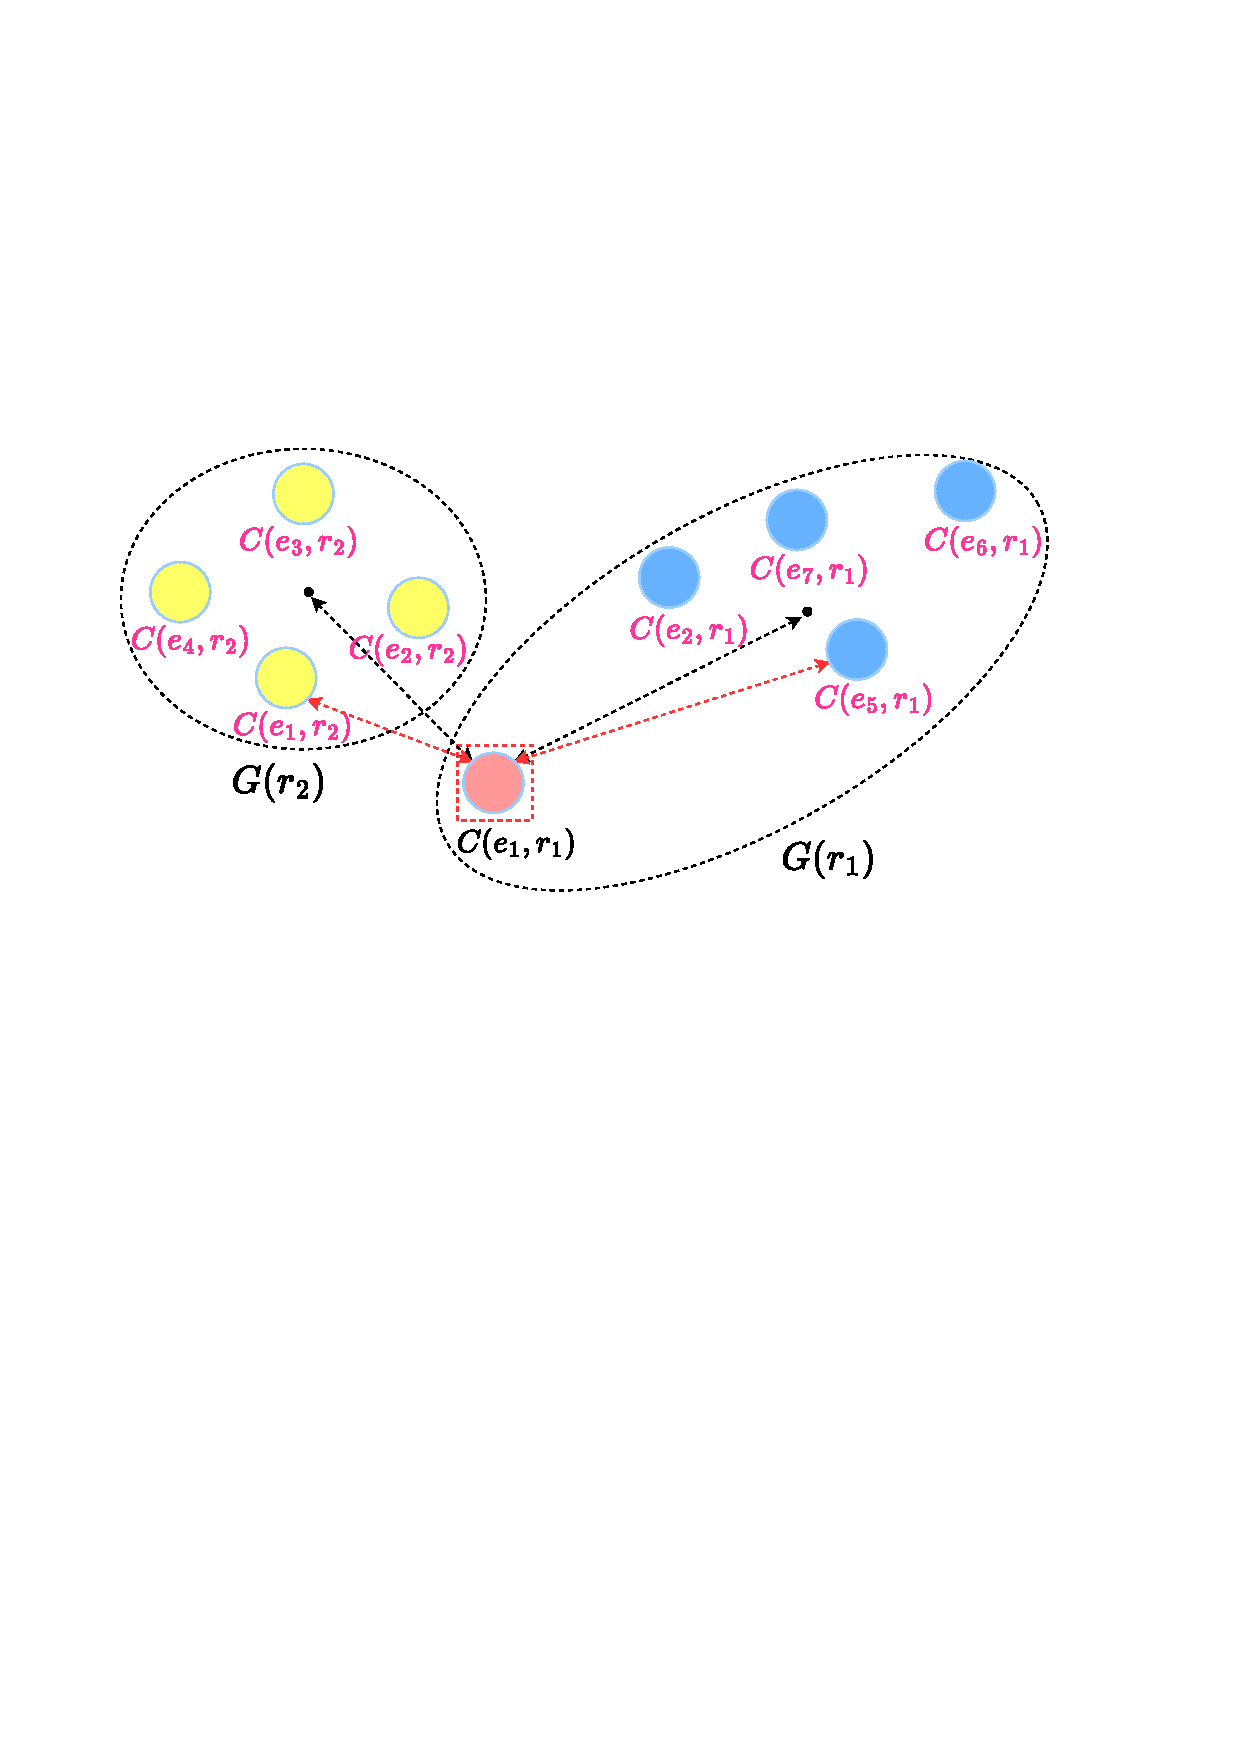
\includegraphics[width=0.7\linewidth]{figures/chap4/overdependence.pdf}
   \caption{实体类型过度依赖示例图}
   \label{fig-overdependence}
\end{figure}

\subsection{预实验验证}
\label{pre_experiment}
基于实体类型过度依赖的定义,本章节通过预实验验证其对于事件要素抽取性能的影响。

\textbf{数据集和模型}~在数据集方面,预实验评估选择了广泛使用的事件检测语料库ACE2005数据集,其具体细节将在主实验章节进行阐述。在模型方面,由于RNN、CNN和BERT是事件要素抽取最常用的三类编码器,预实验基于所选数据集训练了三种不同的事件要素抽取模型,包括AttRNN、DMCNN~\cite{chen2015event}和DMBERT~\cite{wang2019adversarial}。其中,基于RNN的事件要素抽取模型如JRNN~\cite{nguyen2016joint}和dbRNN~\cite{sha2018jointly}未公布源代码,因此本文受Lu等人~\cite{lu2019distilling}研究工作的启发,利用增加了注意力机制的双向LSTM作为使用RNN架构的基线模型,记作AttRNN。此外,由于训练集和测试集之间的数据分布相似,实验中将根据实体类型依赖、语义不一致和实体类型过度依赖的定义,分别评估测试集中相应簇的性能。由于事件要素抽取的测试集依赖于事件检测的预测结果,本文遵循Wang等人和Xi等人~\cite{wang2019hmeae,xiangyu2021capturing}的实验设置,分别使用训练好的AttRNN、DMCNN和DMBERT来检测事件类型和相应的触发词。考虑到测试的实例数量取决于不同事件检测模型正确预测的事件数量,本实验中三种基线模型对应的测试集实例数分别为4013、3630和4081。

\textbf{实验步骤}~首先,对于给定模型,本章使用其编码器获取测试集中每个实例的特征编码表示。然后,基于要素类型,测试集中的所有实例被划分为不同的群组,使得每个群组中实例的要素类型是相同的。进一步地,根据实体类型,将每个群组中的实例划分为不同的簇。因此,同一簇中实例的实体类型和要素类型是相同的。对于AttRNN、DMCNN和DMBERT各自对应的编码器,根据上述划分步骤可分别得到簇的数目为156、148和161。基于此,本章通过简单地计算各个群组/簇中所有实例特征表示的平均值,以用作其整体表示,其避免了引入额外计算参数和降低了计算复杂度。然后,本实验根据实体类型依赖、语义不一致和实体类型过度依赖的定义对每个簇进行判定,并分别计算符合不同定义的测试子集的性能(F1值)。

\textbf{评估验证}~预实验结果如表\ref{performance_pre}所示,其展示了根据不同定义类型划分的测试子集的簇数目及相应性能结果。从表中可以观察到:(1)对于不同的事件要素抽取模型,符合实体类型过度依赖的实例簇的性能都较低。其与其他类型的实例簇之间的巨大性能差异表明,现有事件要素抽取基线模型不擅长处理实体类型过度依赖问题。(2)符合实体类型过度依赖的实例簇和语义不一致的实例簇之间的性能差异表明,与语义不一致相比,由实体类型和要素类型之间的相关性导致的实体类型过度依赖进一步降低了模型的性能。(3)未对实体类型信息过度依赖的簇和整个测试集的性能差异表明,如果事件要素抽取模型缓解了实体类型过度依赖问题,则整体性能可以得到提升。

\begin{table*}[htp]
\footnotesize
\centering
\caption{测试集中不同类型实例簇的数目及性能结果}
\label{performance_pre}
\begin{tabular}{l|ccccc}
\toprule
模型  & \begin{tabular}[c]{@{}c@{}}实体类型依赖\\ (数目/F1 (\%))\end{tabular} & \begin{tabular}[c]{@{}c@{}}语义不一致\\ (数目/F1 (\%))\end{tabular} & \begin{tabular}[c]{@{}c@{}}实体类型过度依赖\\ (数目/F1 (\%))\end{tabular} & \begin{tabular}[c]{@{}c@{}}非实体类型过度依赖\\ (数目/F1 (\%))\end{tabular} & \begin{tabular}[c]{@{}c@{}}所有簇\\ (数目/F1 (\%))\end{tabular} \\ \midrule
AttRNN  & 100 / 40.6  & 56 / 38.9 & 48 / \textbf{18.1} & 108 / 63.6  & 156 / 50.9    \\
DMCNN   & 112 / 46.0 & 76 / 32.6 & 52 / \textbf{15.6} & 96 / 71.4  & 148 / 53.5    \\
DMBERT  & 95 / 38.6 & 48 / 40.7 & 31 / \textbf{15.3} & 130 / 68.9  & 161 / 57.2   \\ \bottomrule
\end{tabular}
\end{table*}

由于不同簇中的实例数量差异较大,本章节进一步统计了符合实体类型过度依赖的簇中实例的数目占据所有测试实例的比例,记作“实体类型过度依赖比例”。表\ref{number_pre}展示了不同事件要素抽取模型的比例结果。本文将在章节\ref{evaluation_section}中评估下一节所提的实体类型过度依赖消解方法是否可以降低“实体类型过度依赖比例”,进而提高整体性能。

\begin{table*}[htp]
\centering
\small
% \setlength{\abovecaptionskip}{0pt}
% \setlength{\belowcaptionskip}{10pt}
\caption{符合实体类型过度依赖的簇中实例统计信息}
\label{number_pre}
\begin{tabular}{l|ccc}
\toprule
模型 & 实体类型过度依赖的簇中实例数 & 总实例数 & 实体类型过度依赖比例(\%) \\ \midrule
AttRNN  & 2845  & 4013  & 70.9  \\
DMCNN   & 2799  & 3630  & 77.1  \\
DMBERT  & 1281  & 4081  & 31.4  \\ \bottomrule
\end{tabular}
\end{table*}

从预实验中可以观察到,实体类型过度依赖问题降低了事件要素抽取模型的整体性能。为了缓解该问题,本文考虑降低“实体类型过度依赖比例”。进一步,其是由实体类型依赖导致,则可以利用以下两种方式处理:(1)增加具有相同要素类型但实体类型不同的实例特征表示之间的相似性;(2)降低具有不同要素类型但实体类型相同的实例特征表示之间的相似性。基于此,下一节将具体介绍将上述两种方式整合的所提方法,从而提高事件要素抽取的性能。

\section{方法设计}
本章将详细介绍基于多角度对比学习的实体类型过度依赖消解方法,其可以应用于不同的事件要素抽取基线模型。为了描述方便,本章选取DMBERT~\cite{wang2019adversarial},以其为基础介绍相应的多角度实体类型过度依赖消解的事件要素抽取模型METOR。图\ref{framework}展示了所提模型的总体架构,其主要由四个模块组成:编码器、正样本处理、负样本处理和循环训练策略。

\begin{figure}[htp]
    \centering
   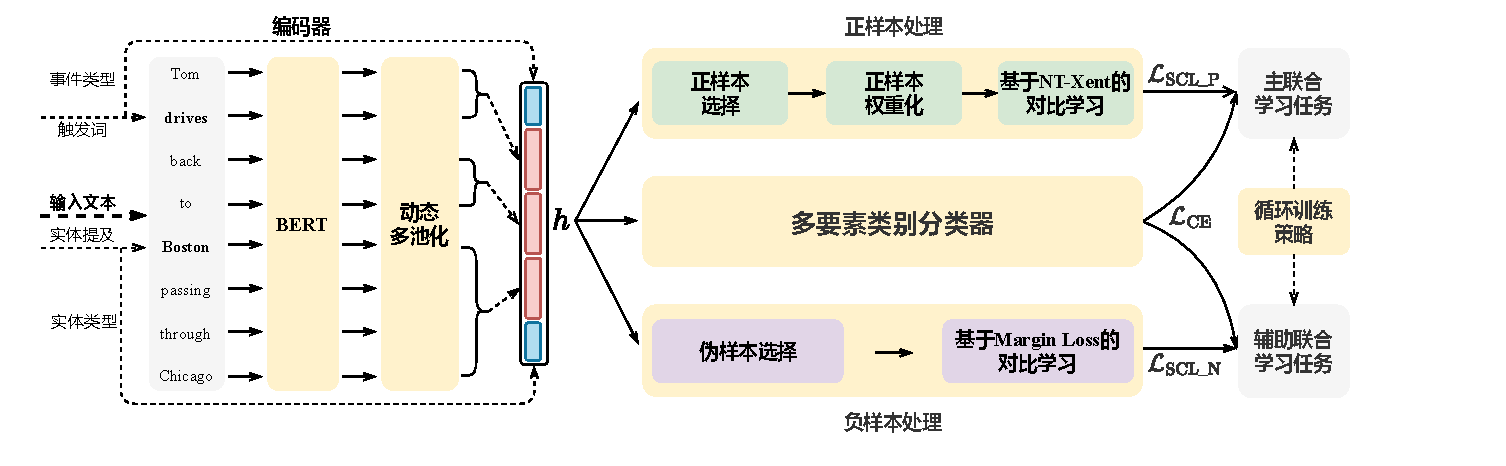
\includegraphics[width=1\linewidth]{figures/chap4/framework_metor.pdf}
   \caption{METOR模型架构图}
   \label{framework}
\end{figure}

\subsection{编码器}
编码器模块旨在将每个实例编码成对应的特征表示。由于事件要素抽取为事件检测的后续任务,本章节遵循Wang等人~\cite{wang2019hmeae}和Xi等人~\cite{xiangyu2021capturing}的研究工作,先利用Wang等人~\cite{wang2019hmeae}提出的DMBERT事件检测模型进行事件触发词和相应事件类型的预测,并将所有实体提及设置为待抽取的事件要素候选。由于句子中可能存在多个事件要素候选,本章将这些候选分成多个实例处理。假设给定的事件要素候选为$arg$,其实体类型为$e$,所参与预测的事件触发词为
$tri$,对应的事件类型为$t$,首先利用BERT~\cite{devlin2019bert}对所在句子文本$x=\left\{w_{1},\cdots,tri,\cdots ,arg, \cdots, w_{n}\right\}$进行编码得到特征表示:
\begin{equation}
  \left\{\boldsymbol{\hat{h}}_{1},\cdots,\boldsymbol{\hat{h}}_{p_{tri}},\cdots,\boldsymbol{\hat{h}}_{p_{arg}},\cdots,\boldsymbol{\hat{h}}_{n}\right\}=\textrm{BERT}(w_{1},\cdots, tri,\cdots, arg, \cdots, w_{n})
\end{equation}
其中$p_{tri}$和$p_{arg}$分别表示$tri$和$arg$在输入句子中的位置。

在此之后,使用一个动态多池化操作分段聚合编码后的特征表示:
\begin{equation}
    \left[\boldsymbol{h}_{1, p_{tri}}\right]_{k}=\max \left\{\left[\boldsymbol{\hat{h}}_{1}\right]_{k} \cdots,\left[\boldsymbol{\hat{{h}}}_{p_{tri}}\right]_{k}\right\}
\end{equation}
\begin{equation}
    \left[\boldsymbol{{h}}_{p_{tri}+1, p_{arg}}\right]_{k}=\max \left\{\left[\boldsymbol{\hat{h}}_{p_{tri}+1}\right]_{k} \cdots,\left[\boldsymbol{\hat{{h}}}_{p_{arg}}\right]_{k}\right\}
\end{equation}
\begin{equation}
    \left[\boldsymbol{{h}}_{p_{arg}+1, n}\right]_{k}=\max \left\{\left[\boldsymbol{\hat{h}}_{p_{arg}+1}\right]_{k} \cdots,\left[\boldsymbol{\hat{{h}}}_{n}\right]_{k}\right\}
\end{equation}
其中$[\cdot]_{k}$表示对应向量的第$k$个值。然后,本章随机初始化所有的事件类型标签和实体类型标签,分别表示为$\boldsymbol{W}_{T} \in {\mathbb{R}}^{n_{t} \times d_{s}}$和$\boldsymbol{W}_{E} \in {\mathbb{R}}^{n_{e} \times d_{s}}$。其中,$d_{s}$、$n_{t}$和$n_{e}$分别表示事件类型(实体类型)向量的维度、预定义的事件类型数目和预定义的实体类型数目。此外,$\boldsymbol{W}_{T}\left(t\right)$表示使用
事件类型$t$从向量矩阵$\boldsymbol{W}_{T}$中查找出的事件类型向量。类似地,$\boldsymbol{W}_{E}\left(e\right)$表示根据实体类型$e$查找出的实体类型向量。最后,串接上述表示,得到实例的特征表示$\boldsymbol{h} \in {\mathbb{R}}^{d_{out}}$如下:
\begin{equation}
\label{input_information}
\boldsymbol{h}=\left[\boldsymbol{h}_{1, p_{tri}};\boldsymbol{{h}}_{p_{tri}+1, p_{arg}};\boldsymbol{{h}}_{p_{arg}+1, n};\boldsymbol{W}_{T}\left(t\right);\boldsymbol{W}_{E}\left(e\right)\right]
\end{equation}

\subsection{正样本处理}
本模块提出了一种选择-加权的对比学习方法,该方法包括三个步骤:正样本选择、正样本加权和基于归一化温度标度交叉熵(NT-Xent)的对比学习。首先,该方法基于给定实例的实体类型选择正样本,使得模型能够聚焦于处理与给定实例的实体类型无关的正样本。然后,计算全局共现信息和语义相关性信息,以对所选正样本的相关性进一步权重化处理。基于此,模型可以提升特定正样本的对比学习贡献,其包含了更多与给定实例要素类型相关的关键语义信息,从而学习到实体类型信息之外的更多有效语义知识。最后,计算基于NT-Xent的选择-加权对比学习方法的训练损失。

\textbf{正样本选择}~给定一批包含$K$个实例的批数据 $\mathcal{B}$,对于其中的每个实例$x_{i}$,首先选择与其要素类型相同的实例作为正样本集合$\mathcal{P}\left(x_{i}\right)$,选择与其要素类型不同的实例作为负样本集合$\mathcal{N}\left(x_{i}\right)$。基于
$\mathcal{P}\left(x_{i}\right)$,本节采用一个简单的选择策略去获取新的正样本集合:
\begin{equation}
  \mathcal{P}_{s}\left(x_{i}\right)=\left\{x_{p}: x_{p} \in \mathcal{B}, (e_{p} \neq e_{i}) \wedge (r_{p}=r_{i}) \wedge (p \neq i)\right\}
\end{equation}
其中$r_{i}$和$e_{i}$分别表示实例$x_{i}$的要素类型和实体类型。本选择策略只用于包含了不止一个样本的$\mathcal{P}\left(x_{i}\right)$,以避免造成对比数据的稀疏。

\textbf{正样本加权}~在完成正样本选择后,本章根据要素类型$r_{i}$,对$\mathcal{P}_{s}\left(x_{i}\right)$中的每个正样本分配一个权重。传统的对比学习方法在对比学习损失中等同地对待所有正样本,无法区分具有不同实体类型的正样本的重要程度。为此,本章基于要素类型$r_{i}$,从全局共现信息和语义相关性信息两个方面,计算不同正样本对于$x_{i}$的重要性。

全局共现信息可表示为记录了整个训练集中不同实体类型和要素类型共现数量的共现矩阵$I_{e,r}$。假设$\mathcal{E}$和$\mathcal{R}$分别为训练集中的实体类型和要素类型集合,批数据$\mathcal{B}$中第$p$个实例(即$x_{p}$)存在于集合$\mathcal{P}_{s}\left(x_{i}\right)$中,其实体类型为$e_{p}$。受TF-IDF~\cite{salton1988term}启发,首先定义实体类型频率(ETF),用于表示$e_{p}$与$r_{i}$同时出现的频率:
\begin{equation}
  {\textrm{ETF}}\left(e_{p}, r_{i}\right)=\frac{I_{e_{p},r_{i}}}{\sum_{m \in \mathcal{E}} I_{m,r_{i}}}
\end{equation}

此外,本章使用与$e_{p}$同时出现的要素类型的数量来衡量$e_{p}$的重要性。要素类型数量越少,$e_{p}$则越重要。因此,反向要素类型频率(IRTF)可根据如下定义得到:
\begin{equation}
  {\textrm{IRTF}}\left(e_{p}\right)=\log \frac{|\mathcal{R}|}{|\{r \in \mathcal{R}: I_{e_{p},r} > 0\}|+1}
\end{equation}

基于ETF和IRTF,可得实例$x_{p}$对于实例$x_{i}$在全局共现信息方面的重要性得分:
\begin{equation}
 w_{1}\left(x_{p}, x_{i}\right)= {\textrm{ETF}}\left(e_{p}, r_{i}\right) \times {\textrm{IRTF}}\left(e_{p}\right)
\end{equation}

然而,在事件类型不同的实例中,具有相同实体类型的实体提及可能以不同的要素类型参与在事件中。因此,对于不同的事件类型,即使实例的实体类型相同,对给定实例的重要性也应有所区分。因此,考虑$x_{p}$对$x_{i}$的重要性时仅使用全局共现信息不足以建模不同事件类型的影响。基于此,本节进一步利用语义相关性信息。首先,将所有要素类型标签随机初始化成向量矩阵$\boldsymbol{W}_{R} \in {\mathbb{R}}^{n_{r} \times d_{s}}$,其中$n_{r}$为预定义的要素类型的数目(包括特殊要素类型“空”),$d_s$是要素类型向量的维度。然后,对于给定的实例$x_{i}$,得到融合事件类型信息的实体类型和要素类型表示:
\begin{equation}
 \boldsymbol{e}_{i}^{t} = \boldsymbol{W}_{T}\left(t_{i}\right) \odot \boldsymbol{W}_{E}\left(e_{i}\right)
 \label{eq9}
\end{equation}
\begin{equation}
 \boldsymbol{r}_{i}^{t} = \boldsymbol{W}_{T}\left(t_{i}\right) \odot \boldsymbol{W}_{R}\left(r_{i}\right)
 \label{eq11}
\end{equation}
其中$\odot$表示元素依次相乘,$r_{i}$、$e_{i}$和$t_{i}$分别表示实例$x_{i}$的要素类型、实体类型和事件类型。$\boldsymbol{W}_{T}\left(t_{i}\right)$表示使用
事件类型$t_{i}$从向量矩阵$\boldsymbol{W}_{T}$中查找出的事件类型向量。类似地,可以分别得到实体类型向量$\boldsymbol{W}_{E}\left(e_{i}\right)$和要素类型向量$\boldsymbol{W}_{R}\left(r_{i}\right)$的含义。由于
$\boldsymbol{W}_{T}$和$\boldsymbol{W}_{E}$同时也是公式\ref{input_information}中串接向量的一部分,事件类型和实体类型的语义信息实现了在不同模块间的共享。同样,可以得到任意正样本$x_{p}$的融合事件类型信息的实体类型表示$\boldsymbol{e}_{p}^{t}$。然后,本章基于语义相关性信息,利用注意力机制计算$x_{p}$对于$x_{i}$的重要性得分,并根据$\textrm{softmax}$函数得到归一化结果$w_{2}\left(x_{p}, x_{i}\right)$:
\begin{equation}
s\left(x_{p},x_{i}\right)=\boldsymbol{v}^{\top} \tanh \left(\boldsymbol{U}\left[\boldsymbol{e}_{i}^{t};\boldsymbol{e}_{p}^{t};\boldsymbol{r}_{i}^{t}\right]\right)
\end{equation}
\begin{equation}
 w_{2}\left(x_{p}, x_{i}\right) =  \frac{\exp \left(s\left(x_{p},x_{i}\right)\right)}{\sum_{e_{j} \in \mathcal{E}}\exp \left(s\left(x_{j},x_{i}\right)\right)}
\end{equation}
其中$\boldsymbol{v} \in {\mathbb{R}}^{3d_{s}}$和$\boldsymbol{U} \in {\mathbb{R}}^{3d_{s} \times 3d_{s}}$分别表示可训练学习的向量和矩阵参数。然后,可得$x_{p}$对于$x_{i}$的最终重要性得分:
\begin{equation}
 {\textrm{w}}\left(x_{p}, x_{i}\right) = \alpha w_{1}\left(x_{p}, x_{i}\right) + (1-\alpha) w_{2}\left(x_{p}, x_{i}\right)
\end{equation}
其中$\alpha\,(0 < \alpha < 1)$为权重参数。

\textbf{基于NT-Xent的对比学习}~遵循Chen等人~\cite{chen2020simple}和Khosla等人~\cite{khosla2020supervised}的研究,本章首先将实例$x_{i}$的特征表示$\boldsymbol{h}_{i}$映射到一个新空间上,以提高对比学习的质量:
\begin{equation}
\label{map}
  \boldsymbol{z}_{i}=\boldsymbol{W}_{1} f\left(\boldsymbol{W}_{2} \boldsymbol{h}_{i}\right)
\end{equation}
$\boldsymbol{W}_{1} \in {\mathbb{R}}^{d_{1} \times d_{2}}$和$\boldsymbol{W}_{2} \in {\mathbb{R}}^{d_{2} \times d_{out}}$为可训练学习的矩阵参数,$f(\cdot)$为ReLU激活函数,其中$d_{1}$和 $d_{2}$为维度参数。在选择出正样本并对其权重化后,本章基于NT-Xent~\cite{chen2020simple}计算相应的对比学习损失$\mathcal{L_\textrm{SCL\_P}}$如下:
\begin{equation}
\label{nt_loss}
\mathcal{L_\textrm{SCL\_P}}=\sum_{i=1}^{K} \frac{-1}{|\mathcal{P}_{s}\left(x_{i}\right)|} \sum_{p \in \mathcal{P}_{s}\left(x_{i}\right)} {\textrm{w}}(x_{p}, x_{i}) \cdot \log \frac{\exp \left(\textrm{sim}\left(\boldsymbol{z}_{i},\boldsymbol{z}_{p}\right) / \tau\right)}{\sum_{n \in K\backslash i }\exp \left(\textrm{sim}\left(\boldsymbol{z}_{i},\boldsymbol{z}_{n}\right) / \tau\right)}
\end{equation}
其中$\textrm{sim}\left(\boldsymbol{z}_{i},\boldsymbol{z}_{p}\right)=\boldsymbol{z}_{i}^\top\boldsymbol{z}_{p}/\lVert\boldsymbol{z}_{i}\rVert \,\lVert\boldsymbol{z}_{p}\rVert$,$\tau$表示温度参数。

\subsection{负样本处理}
本模块提出了一种伪正对比学习方法,该方法包括两个步骤:伪样本选择和基于边际损失(Margin Loss)的对比学习。首先,基于实体类型从负样本中选择出伪正样本。然后,利用这些选择出的样本作为对比参考,降低给定实例和与其实体类型相同的负样本之间的特征表示相似性。

\textbf{伪样本选择}~给定一批包含$K$个实例的批数据$\mathcal{B}$,对于其中的每个实例$x_{i}$,首先选择对应的伪正样本和伪负样本,选择过程如下:
\begin{equation}
  \mathcal{P}_{pseudo}\left(x_{i}\right)=\left\{x_{p}: x_{p} \in \mathcal{B}, (e_{p} \neq e_{i}) \wedge (r_{p} \neq r_{i}) \wedge (p \neq i)\right\}
\end{equation}
\begin{equation}
  \mathcal{N}_{pseudo}\left(x_{i}\right)=\left\{x_{n}: x_{n} \in \mathcal{B}, (e_{n}=e_{i}) \wedge (r_{n} \neq r_{i}) \wedge (n \neq i)\right\}
\end{equation}
其中伪正样本集合和伪负样本集合分别表示为 $\mathcal{P}_{pseudo}\left(x_{i}\right)$和 $\mathcal{N}_{pseudo}\left(x_{i}\right)$。

\textbf{基于边际损失的对比学习}~
首先,本章计算$\mathcal{P}_{pseudo}\left(x_{i}\right)$和 $\mathcal{N}_{pseudo}\left(x_{i}\right)$中实例特征表示的平均值,分别得到$\boldsymbol{z}_{i}^{P}$和$\boldsymbol{z}_{i}^{N}$,以表示这两个集合的整体信息。然后,利用$\mathcal{P}_{pseudo}\left(x_{i}\right)$作为对比参考进行对比学习,以降低实例$x_{i}$与属于$\mathcal{N}_{pseudo}\left(x_{i}\right)$的样本之间的相似性。由于$\mathcal{P}_{pseudo}\left(x_{i}\right)$中的样本本质上仍是$x_{i}$的负样本,使用实例级的对比学习损失NT-Xent以增加伪正样本与给定实例之间的相似性是不合适的。因此,本章使用边际损失来对伪正样本集合和伪负样本集合的整体表示进行对比学习:
\begin{equation}
\label{eq21}
  \mathcal{L_\textrm{SCL\_N}} =\sum_{i=1}^{K} \max \left\{\boldsymbol{z}_{i}^{N} \cdot \boldsymbol{z}_{i}-\boldsymbol{z}_{i}^{P} \cdot \boldsymbol{z}_{i}+\gamma, 0\right\}
\end{equation}
其中$\gamma$为边际超参数。

\subsection{循环训练策略}
本模块首先计算事件要素抽取任务的损失。给定实例$x$,将其从编码器模块得到的特征表示\boldsymbol{$h$}输入到多要素类别分类器,以计算概率分布$p\left(x\right)$如下:
\begin{equation}
  p\left(x\right) = \textrm{softmax}\left(\boldsymbol{W}^{c}\boldsymbol{h} + \boldsymbol{b}^{c}\right)
 \label{eq3}
\end{equation}
其中$\boldsymbol{W}^{c} \in {\mathbb{R}}^{n_{r} \times d_{out}}$和$\boldsymbol{b}^{c} \in {\mathbb{R}}^{n_{r}}$分别表示分类器中要训练的参数。给定包含$K$个实例的批数据$\mathcal{B}$,交叉熵损失$\mathcal{L_\textrm{CE}}$计算如下:
\begin{equation}
  \mathcal{L_\textrm{CE}} = -\sum^{K} \log p\left(r|x\right)
 \label{ce}
\end{equation}
其中$p\left(r|x\right)$表示将实例$x$预测为正确的要素类型$r$的概率值。在测试阶段,$p\left(x\right)$用于获取事件要素抽取的预测要素类型。

进一步,本章注意到优化$\mathcal{L_\textrm{SCL\_N}}$将不可避免地提升实例$x_{i}$和$\mathcal{P}_{pseudo}\left(x_{i}\right)$中的样本(本质上为负样本)间的特征表示相似度。然而,根据公式\ref{nt_loss},优化$\mathcal{L_\textrm{SCL\_P}}$会降低实例$x_{i}$和所有负样本间的特征表示相似度。因此, $\mathcal{L_\textrm{SCL\_N}}$和$\mathcal{L_\textrm{SCL\_P}}$的训练目标是不一致的。为此,本章提出了一个循环训练策略,该策略依次使用两个不同的联合训练目标来协调$\mathcal{L_\textrm{SCL\_P}}$和 $\mathcal{L_\textrm{SCL\_N}}$的不一致。具体来说,将联合优化$\mathcal{L_\textrm{SCL\_P}}$和 $\mathcal{L_\textrm{CE}}$视作主联合学习任务,先训练$f$轮,其中$f$是超参数。然后,将联合优化$\mathcal{L_\textrm{SCL\_N}}$和 $\mathcal{L_\textrm{CE}}$视作辅助联合学习任务,再训练一轮。重复上述过程直到训练完成。通过这种方式,可以逐步调整处理$\mathcal{L_\textrm{SCL\_P}}$和$\mathcal{L_\textrm{SCL\_N}}$训练目标的不一致。本章提出的训练策略表示如下:
\begin{equation}
\label{eq24}
\mathcal{L_\textrm{JOINT}}=\left\{\begin{array}{lr}
 \mathcal{L_\textrm{SCL\_P}}+\mathcal{L_\textrm{CE}} & epoch \bmod f \neq 0 \\
 \mathcal{L_\textrm{SCL\_N}}+\mathcal{L_\textrm{CE}} & epoch \bmod f = 0 
\end{array}\right.
\end{equation}
其中$epoch$表示完成训练的轮次。

\section{实验评估}
\label{evaluation_section}
在实验评估中,本章所提的方法不仅应用于基线模型DMBERT,也应用于AttRNN和DMCNN基线模型,分别记作METOR(RNN)和METOR(CNN)。在METOR(RNN)和METOR(CNN)中,将编码器模块中的DMBERT分别替换为AttRNN和DMCNN,其他模块保持不变。由于事件要素抽取任务依赖于事件检测的结果,本章遵循Wang等人~\cite{wang2019hmeae}和Xi等人~\cite{xiangyu2021capturing}的研究设定,使用经过训练的AttRNN、DMCNN和DMBERT分别检测事件触发词和相应的事件类型,作为METOR(RNN)、METOR(CNN)和METOR模型的输入。接下来,本章将介绍实验设置、性能结果、消融研究、实体类型信息深入分析、超参数敏感性分析、计算复杂性分析和案例研究。

\subsection{实验设置}
\label{settings_4}
\textbf{1.数据集}~遵循最近主流的给定实体提及的事件要素抽取研究工作~\cite{xiangyu2021capturing,liu2018jointly, nguyen2016joint},本章实验评估在ACE2005数据集上进行。与章节\ref{experiment_settings}相同,其为ACE2005语料库~\cite{doddington2004automatic}中的英文版本数据集。根据Wang等人~\cite{wang2019hmeae}的预处理设置\footnote{https://github.com/thunlp/HMEAE},该数据集包含599个文档、33种事件类型、46种实体类型和35种事件要素类型。此外,引入$None$(空)作为特殊要素类型,以表示相应的候选要素在给定实例中为非事件要素。进一步,该数据集被划分为529、30和40个文档,分别作为训练集、验证集和测试集。

\textbf{2.评价指标}~本章实验遵循事件要素抽取任务的标准评估。如果事件类型、偏移量和要素类型与数据集的标注完全相同,则认定候选要素被正确抽取,其中偏移量指候选要素文段在句子中的开始和结束位置索引。基于此,本文使用准确率(P)、召回率(R)和F1值(F1)作为评估指标,其计算方式参照章节\ref{experiment_settings}。

\textbf{3.实验配置}~在编码器模块中,对于METOR(RNN)本章使用预训练Glove词向量、随机初始化事件类型向量、随机初始化实体类型向量和随机初始化位置向量,维度分别为100、5、5和5,并在模型中使用双向LSTM和自注意力机制。对于METOR(CNN),使用与DMCNN相同的输入向量和超参数。类似地,本章将5维随机初始化的实体类型向量添加到METOR(CNN)的输入中。对于METOR,编码使用的BERT预训练模型为HuggingFace发布的“google-bert/bert-base-uncased”版本\footnote{https://huggingface.co/google-bert/bert-base-uncased},实体类型向量维度$d_{s}$设置为50。在正样本处理模块中,本章将$d_{1}$设置为512,$d_{2}$设置为512,温度参数$\tau$设置为0.1,权重$\alpha$设置为0.7。在负样本处理模块中,将$\gamma$设置为0.1。在循环训练策略中,METOR(RNN)、METOR(CNN)和METOR的循环频率$f$分别设置为4、3和3。此外,其批数据大小均设置为80,训练轮次设置为10,优化器使用AdamW,对应的学习率分别设置为$1 \times 10^{-3}$, $1 \times 10^{-3}$和$5 \times 10^{-5}$。对于不同的模型,训练均在相同实验服务器上进行,具体配置为:CPU型号Intel(R) Xeon(R) Gold 5320,主频2.20GHz;内存256G;GPU计算卡型号NVIDIA GeForce RTX 3090,显存24G。上述模型均基于Pytorch~\cite{paszke2017automatic}框架进行构建。

\textbf{4.基线模型}~本节选择以下模型作为实验比较的基线:

\begin{itemize}
\item DMCNN \cite{chen2015event} - 该模型使用了CNN和动态多池化操作提取实例的特征表示。
\item JRNN \cite{nguyen2016joint} - 该模型提出了包含离散二元矩阵的RNN,其利用了事件类型和要素类型、要素类型间的相互依赖性。
\item dbRNN \cite{sha2018jointly} - 该模型在RNN中引入了依存句法信息,并构建事件内候选要素间的交互向量以捕捉其关联性。
\item DMBERT \cite{wang2019adversarial} - 该模型使用了BERT和动态多池化操作来提取实例的特征表示。
\item PLMETOR \cite{yang2019exploring} - 该模型基于BERT来预测事件要素类型并生成额外的训练实例,以进一步提高性能。
\item HMEAE \cite{wang2019hmeae} - 该模型提出了一种利用事件要素类型语义相关性的层次模块化注意力网络。
\item BERT (Inter) \cite{xiangyu2021capturing} - 该模型基于BERT并利用了跨事件的相互依赖关系
~\cite{nguyen2016joint}。
\item BERT (Intra) \cite{xiangyu2021capturing} - 该模型基于BERT并利用了事件内部的要素依赖关联~\cite{sha2018jointly}。 
\item BERD \cite{xiangyu2021capturing} - 该模型提出了一种能够利用事件内其他要素的类型预测语义信息的的编码器-解码器框架。
\end{itemize}

本章注意到RCEE\_ER~\cite{liu2020event}在F1指标上取了优秀的性能表现,但其受益于额外的数据增广和无监督数据。因此,本章遵循Xi等人~\cite{xiangyu2021capturing}在BERD模型中的基线模型设置,未将RCEE\_ER模型作为实验性能比较的基线。此外,本章将ChatGPT在ACE2005数据集上的性能评估保留到章节\ref{section_5_3}进行展示与分析。

\subsection{性能结果}

表\ref{overall_4_4}展示了本章所提方法与基线模型在ACE2005数据集上的性能结果,其中$\dagger$表示将本章提出的方法应用在DMBERT基线模型时,其性能在双侧$t$检验下显著($p < 0.01$)优于之前性能最优的事件要素抽取模型BERD。根据结果可进一步观察到,与AttRNN相比,METOR(RNN)在F1指标上实现了3.9\%的性能提升。即使与利用了事件类型和要素类型、要素类型间的相互依赖性的JRNN相比,METOR(RNN)也取得了相差无几的F1指标结果。此外,dbRNN的F1指标显著优于METOR(RNN),本文将其归因于两个原因:(1)dbRNN利用了额外的句法信息。(2)dbRNN同时优化了事件检测和事件要素抽取任务的性能,而METOR(RNN)没有受益于这种联合优化。当本章提出的方法应用在DMCNN时,METOR(CNN)相比该基线在F1指标上实现了5\%的提升,比同样使用了DMCNN作为编码器的HMEAE(CNN)提升了2.8\%。并且,METOR(CNN)的F1指标优于大多数没有使用预训练模型的事件要素抽取模型,并与dbRNN相比时展现了相当的性能结果。同时,可以观察到METOR(CNN)的性能优于使用了BERT预训练模型作为编码器的DMBERT、PLMETOR和BERT(Inter)。

当在编码器模块使用DMBERT时,METOR取得了当前最优的F1性能
% {我们注意到,2020年提出的在F1评分中达到了63.6\%。然而,RCEE得益于额外的资源,包括数据论证和无监督数据。因此,我们遵循BERD于2021年提出的模型,并且不将我们提出的模型与RCEE模型进行比较,因为两者在使用外部资源方面存在差异。)(在F1中)
,且相比于之前性能最优的BERD模型提升了2.1\%。此外,METOR的F1指标比相应的DMBERT基线高出了5.2\%。总的来说,由于本章所提的METOR模型可以学习到除实体类型之外的更多语义信息,从而消解了实体类型过度依赖问题,实现了在事件要素抽取任务上对所有基线模型的性能超越。

\begin{table}[htp]
\centering
% \small
% \setlength{\abovecaptionskip}{0pt}
% \setlength{\belowcaptionskip}{10pt}
\caption{ACE2005数据集上的事件要素抽取性能结果}
% $\textrm{METOR}_{avg}$ is the average performance of METOR and $\pm$ represents the standard deviation when five different random seeds are used. 
% $\dagger$ denotes that our model significantly outperforms the best baseline BERD with $p < 0.01$ under a paired two-sided t-test.}
\label{overall_4_4}
\begin{tabular}{lccc}
\toprule
\multicolumn{1}{l|}{模型}       & P(\%)                          & R(\%)                          & F1(\%)                         \\ \midrule
\multicolumn{1}{l|}{AttRNN}        & 50.6                           & 51.1                           & 50.9                         \\
\multicolumn{1}{l|}{DMCNN}        & 62.2                           & 46.9                           & 53.5                           \\
\multicolumn{1}{l|}{JRNN}         & 54.2                           & 56.7                           & 55.4                           \\
\multicolumn{1}{l|}{dbRNN}        & \textbf{66.2}                & 52.8                           & 58.7                           \\
\multicolumn{1}{l|}{HMEAE (CNN)}  & 57.3                           & 54.2                           & 55.7                           \\
\multicolumn{1}{l|}{\textbf{METOR (RNN)}}   & 51.9      &  58.0      &  54.8 \\
\multicolumn{1}{l|}{\textbf{METOR (CNN)}}   & 56.2      & 61.1     & 58.5  \\ \midrule
+ BERT ($base$)               &                                &                                &                                \\ \midrule
\multicolumn{1}{l|}{DMBERT}       & 58.8                           & 55.8                           & 57.2                           \\
\multicolumn{1}{l|}{PLMETOR}        & 62.3                           & 54.2                           & 58.0                           \\
\multicolumn{1}{l|}{BERT (Inter)} & 58.4                           & 57.1                           & 57.8                           \\
\multicolumn{1}{l|}{BERT (Intra)} & 56.4                           & 61.2                           & 58.7                           \\
\multicolumn{1}{l|}{HMEAE (BERT)} & 62.2                           & 56.6                           & 59.3                           \\
\multicolumn{1}{l|}{BERD}         & 59.1                           & 61.5                           & 60.3                           \\
\multicolumn{1}{l|}{\textbf{METOR}} & 60.3                           & $\boldsymbol{64.7}$          &$\boldsymbol{62.4^{\dagger}}$ \\
\bottomrule
% \multicolumn{1}{l|}{$\textbf{METOR}_{avg}$} & $60.14\pm1.16$                            & 64.36$\pm$0.60          &$62.14\pm0.56^{\dagger}$  \\
% \midrule
\end{tabular}
\end{table}

\subsection{消融研究}
本章通过消融研究分析所提方法中每个模块的有效性,包括正样本处理(Positive Sample Processing)、负样本处理(Negative Sample Processing)和循环训练策略(Cyclic Training Strategy),其中$\Delta$ F1表示与完整方法在F1指标上的性能差距。如表\ref{ablation}所示,将本章所提的方法应用到不同的基线模型上,三个模块都能提升相应基线模型的性能。本节选择METOR模型进行着重讨论。首先,如果移除正样本处理和负样本处理模块,METOR模型在F1指标上的性能将分别下降2.0\%和1.3\%,这表明从正样本和负样本角度消解实体类型过度依赖都可以有效地提升事件要素抽取性能。其次,如果将不同模块的损失直接求和并进行联合训练,以替代循环训练策略,则METOR模型在F1上的性能将下降2.9\%。这表明循环训练策略可以有效地调和正样本处理模块和负样本处理模块中的不同对比学习目标。此外,可以观察到即使移除掉正样本处理模块或负样本处理模块,METOR模型仍优于之前性能最优的BERD模型。本文将其归因于这两个模块都推动了模型学习除实体类型之外的更多语义信息,从而消解了实体类型过度依赖问题,提升了整体性能。

\begin{table*}[htp]
\centering
% \setlength{\abovecaptionskip}{0pt}
% \setlength{\belowcaptionskip}{10pt}
\caption{ACE2005数据集上的消融研究结果}
% $\Delta$ F1 is the performance difference in F1 when compared with the full model.}
\label{ablation}
\begin{tabular}{l|cccc}
\toprule
模型 & P(\%) & R(\%) & F1(\%) &$\Delta$ F1\\ 
\midrule
\textbf{METOR (RNN)} & 51.9      &  58.0      &  54.8  & -\\
w/o Positive Sample Processing & 48.7  & 55.7  & 52.0  & -2.8\\
w/o Negative Sample Processing & 51.1  & 57.2  & 54.0   & -0.8\\
w/o Cyclic Training Strategy & 50.8  & 52.7  & 51.7    & -3.1\\ 
\midrule
\textbf{METOR (CNN)} & 56.2      & 61.1      & 58.5  & -\\
w/o Positive Sample Processing & 52.9  & 59.2  & 55.9   & -2.6\\
w/o Negative Sample Processing & 57.4  & 56.3  & 56.8   & -1.7\\
w/o Cyclic Training Strategy & 54.0  & 57.4  & 55.7    & -2.8\\ 
\midrule
\textbf{METOR} & 60.3  & 64.7  & 62.4   & -\\
w/o Positive Sample Processing & 59.7      &  61.2     &  60.4      & -2.0\\
w/o Negative Sample Processing & 59.3  & 62.9  & 61.1   & -1.3\\ 
w/o Cyclic Training Strategy & 57.1  & 62.1  & 59.5   & -2.9\\  
\bottomrule
\end{tabular}
\end{table*} 

\subsection{实体类型信息分析}
作为基于实体的任务,实体类型信息对于事件要素抽取任务的影响是多方面的。一方面,实体类型是事件要素抽取任务中实体提及的主要信息来源。另一方面,其导致事件要素抽取模型产生了实体类型过度依赖,进而降低了模型的整体性能。因此,本节将对实体类型信息进行深入全面的分析。

\textbf{不同变体模型的实体类型信息利用效率分析}~本节设计两种变体模型作为额外的比较基线,即“Baseline+type”和“Baseline+type+CL”,其中“Baseline”可以为AttRNN、DMCNN或DMBERT。具体地,“Baseline”模型不使用实体类型信息,而“Baseline+type”使用实体类型信息作为输入的一部分。此外,对于“Baseline+type+CL”,其除了使用实体类型信息作为输入外,还引入监督对比学习方法~\cite{khosla2020supervised}损失,与公式\ref{ce}中的交叉熵损失直接求和后并进行联合训练。

表\ref{analysis}展示了本章提出的方法与不同变体模型的性能比较。可以观察到,当“Baseline”为AttRNN、DMCNN和DMBERT时,“Baseline+type”在F1指标上的性能与其相比分别提升了0.8\%、1.2\%和1.2\%。这表明在事件要素抽取基线模型的输入中利用实体类型信息,其性能能够得到一定的提升。此外,当“Baseline”为DMCNN和DMBERT时,“Baseline+type+CL”可以进一步提高“Baseline+type”在F1指标上的性能,分别为0.2\%和0.6\%,其表明传统的监督对比学习方法可以进一步提高基线模型利用实体类型信息的效率。进一步,由于METOR模型使用了实体类型信息并针对该信息设计了多角度对比学习方法,使得其能在利用实体类型信息的同时,从文本中学习到除实体类型信息之外的更多语义信息。因此,与AttRNN、DMCNN和DMBERT相比,METOR模型在F1上的性能分别提升了3.9\%、5.0\%和5.2\%。

\begin{table}[htp]
\centering
% \setlength{\abovecaptionskip}{0pt}
% \setlength{\belowcaptionskip}{10pt}
\caption{ACE2005数据集上不同变体模型的性能结果对比}
\label{analysis}
\begin{tabular}{l|cccc}
\toprule
模型  & P(\%) & R(\%) & F1(\%) & $\Delta$ F1\\ \midrule
AttRNN  & 50.6  & 51.1 & 50.9 & -  \\
AttRNN+type & 51.8 & 51.6  & 51.7 & +0.8\\
AttRNN+type+CL & 50.2 & 53.4  & 51.7 & +0.8\\ 
\textbf{METOR (RNN)}  & 51.9  &  58.0 &  54.8  & +3.9\\
\midrule
DMCNN  & 62.2  & 46.9  & 53.5 & - \\
DMCNN+type  & 51.5  & 58.3  & 54.7 & +1.2\\
DMCNN+type+CL & 53.8  & 56.1  & 54.9  &  +1.4\\ 
\textbf{METOR (CNN)} & 56.2 & 61.1 & 58.5 & +5.0\\
\midrule
DMBERT & 58.8  & 55.8 & 57.2 & - \\
DMBERT+type & 55.7  & 61.3  & 58.4 & +1.2\\
DMBERT+type+CL &  55.9 & 62.4  &  59.0  & +1.8\\ 
\textbf{METOR} & 60.3  & 64.7  & 62.4  & +5.2\\
\bottomrule
\end{tabular}
\end{table}

\textbf{实体类型过度依赖程度分析}~在章节\ref{two}中,
可以得知不同的事件要素抽取基线模型均存在实体类型过度依赖问题。如果反映实体类型过度依赖程度的“实体类型过度依赖比例”指标降低,则对应的整体性能也会提升。为了直观验证本章提出的方法在解决实体类型过度依赖问题上的有效性,本节将基于“实体类型过度依赖比例”指标进行具体分析。如图\ref{fig-comparison}所示,与相应的“Baseline”模型相比,“Baseline+type+CL”的“实体类型过度依赖比例”均略有下降,表明普通监督对比学习可以在一定程度上消解实体类型过度依赖问题。进一步,可以观察到将本章提出的方法应用到不同的基线模型时,与相应的“Baseline”模型相比,其“实体类型过度依赖比例”均显著下降。因此,本章所提方法可以有效降低对实体类型的过度依赖程度。此外,可以观察到“Baseline+type+CL”在处理实体类型过度依赖问题的有效性不如本章所提方法,其原因为普通的监督对比学习主要解决定义\ref{definition2}中的语义不一致问题,而没有聚焦于消解实体类型过度依赖问题。

\begin{figure}[htp]
\centering
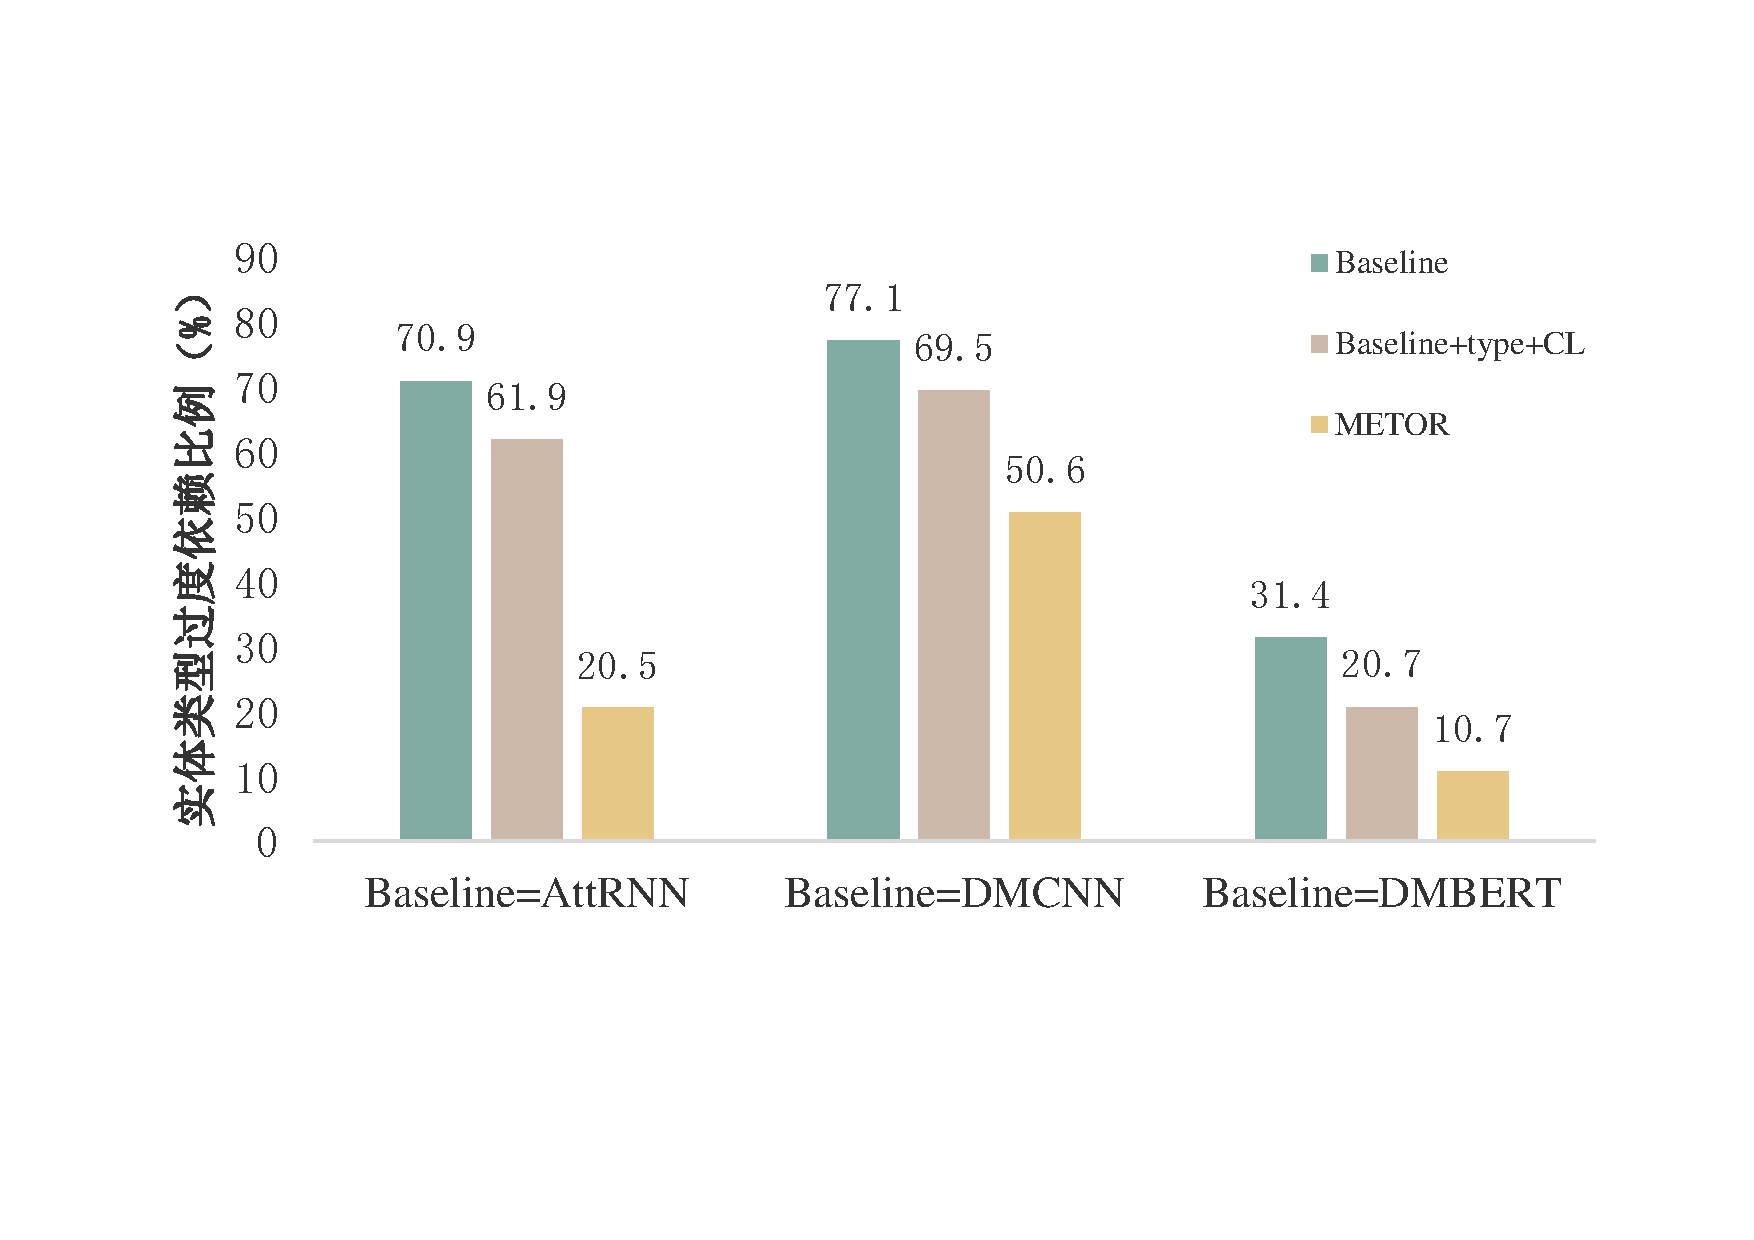
\includegraphics[width=0.8\linewidth]{figures/chap4/comparison.pdf}
\caption{不同模型的实体类型过度依赖程度比较}
\label{fig-comparison}
\end{figure}

\subsection{超参数敏感性分析}
本章分析不同超参数对METOR模型性能的影响,包括公式\ref{nt_loss}中的温度参数$\tau$、公式\ref{eq21}中的边际参数$\gamma$和公式\ref{eq24}中的循环训练频率$f$。

如图\ref{temperature}所示,METOR模型在温度参数$\tau$为0.1时性能最佳。当其在0.02到0.5的范围内变化时,METOR模型的F1性能变化幅度不超过1.1\%,这证明了METOR模型在不同$\tau$的设置下的鲁棒性。

从图\ref{margin}中可以观察到,当边际参数$\gamma$设置为0.1时,METOR模型的F1指标性能达到最佳。当边际参数$\gamma$设置为0.05时,从负样本角度消解实体类型过度依赖问题的程度存在不足,METOR模型的F1的性能略有下降。而当边际参数 $\gamma$大于0.1时,其性能也会下降。这是由于给定实例和伪正样本集合中的负样本之间的特征表示过度相似,导致正样本处理模块和负样本处理模块间的训练目标差距较大。然而,由于METOR模型中的循环训练策略能够极大缓解由较大边际参数$\gamma$引起的训练目标不一致性问题,其性能的下降较为有限。

从图\ref{frequency}中可以观察到,当循环训练频率$f$设置为3时,METOR模型实现了最佳性能。当循环频率$f$设置为2时,循环训练策略中主任务和辅助任务的训练频率没有差异,导致METOR模型在两个不一致的训练目标间频繁切换,从而性能出现下降。此外,当循环频率$f$大于3时,导致循环训练策略中负样本处理模块的训练频率较低,其将接近于退化为不包含负样本处理模块的METOR模型。

\begin{figure*}[t]
\centering
\subfigure[]{
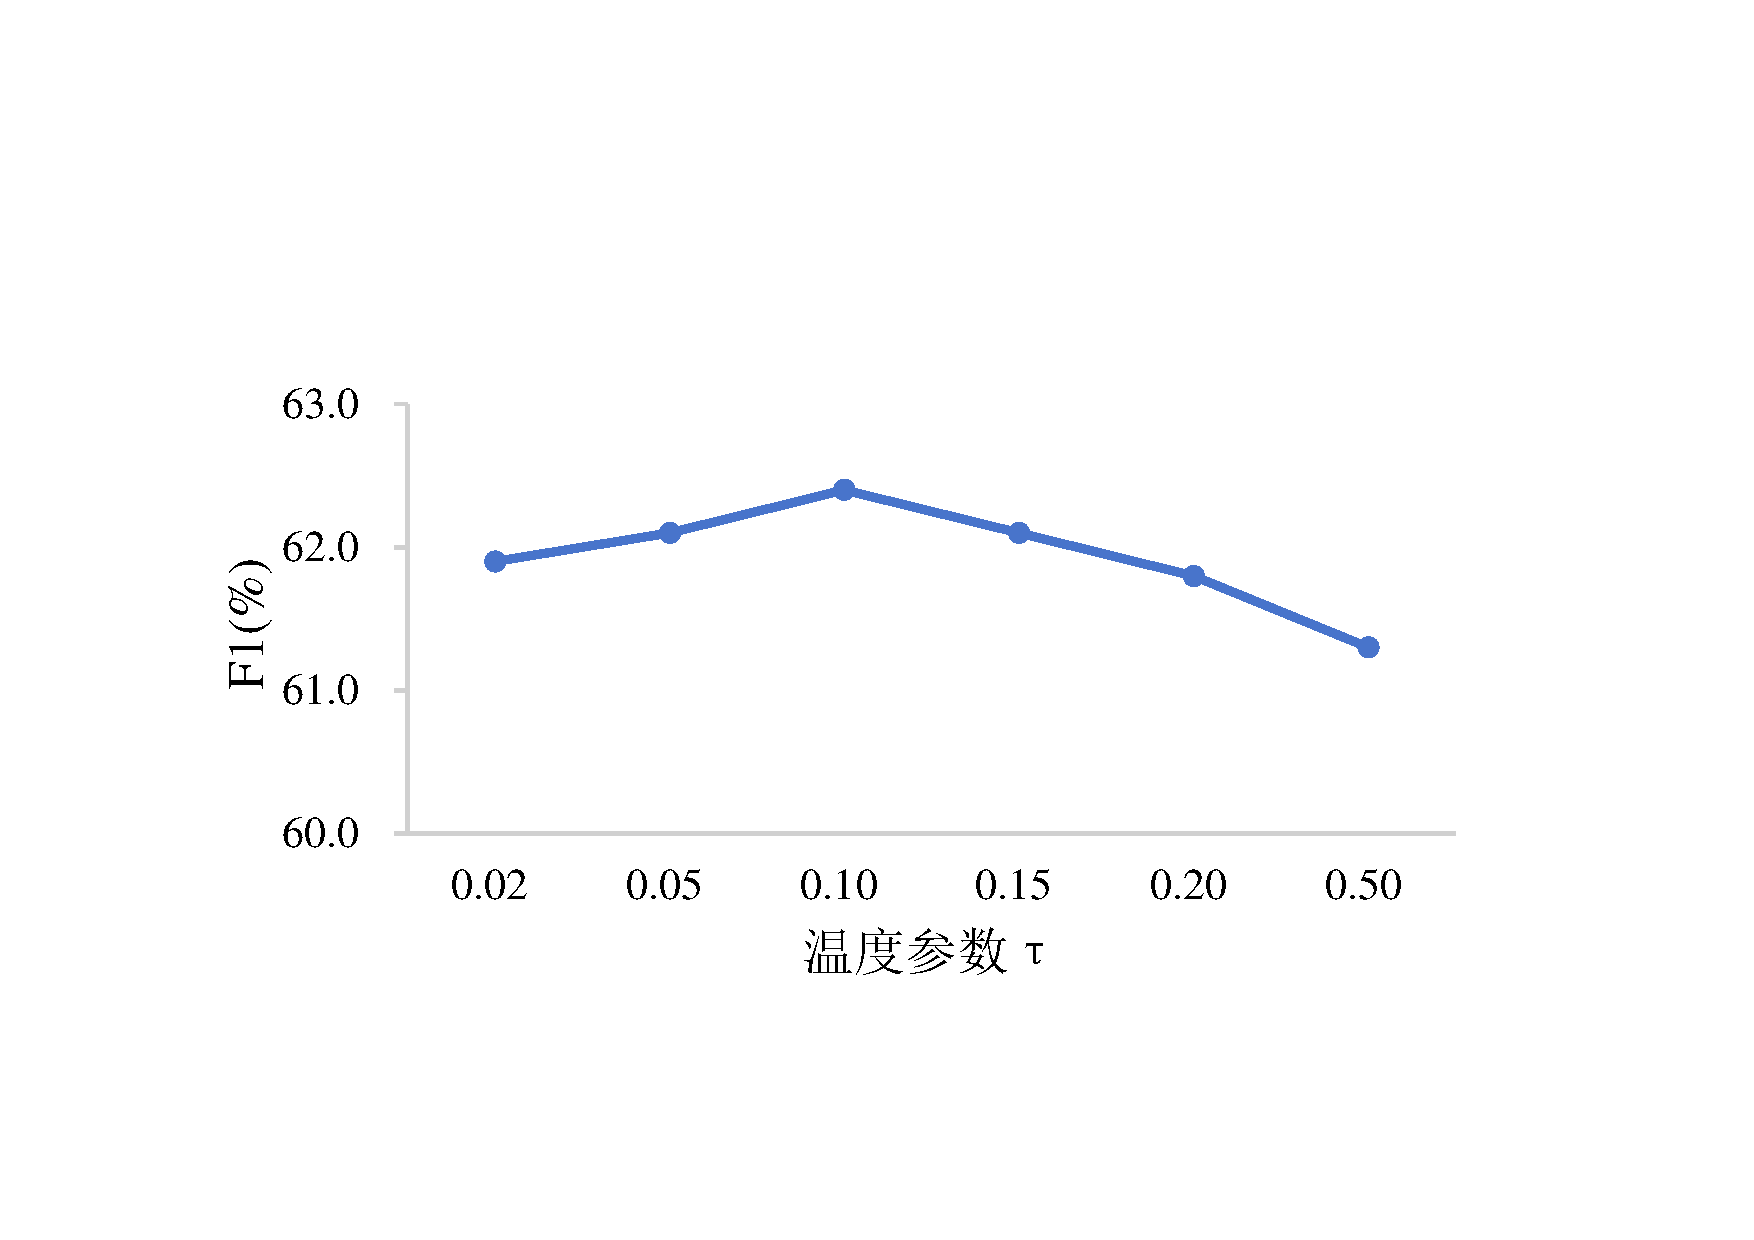
\includegraphics[width=0.6\linewidth]{figures/chap4/temperature.pdf}
\label{temperature}
%\caption{fig1}
}
\quad
\subfigure[]{
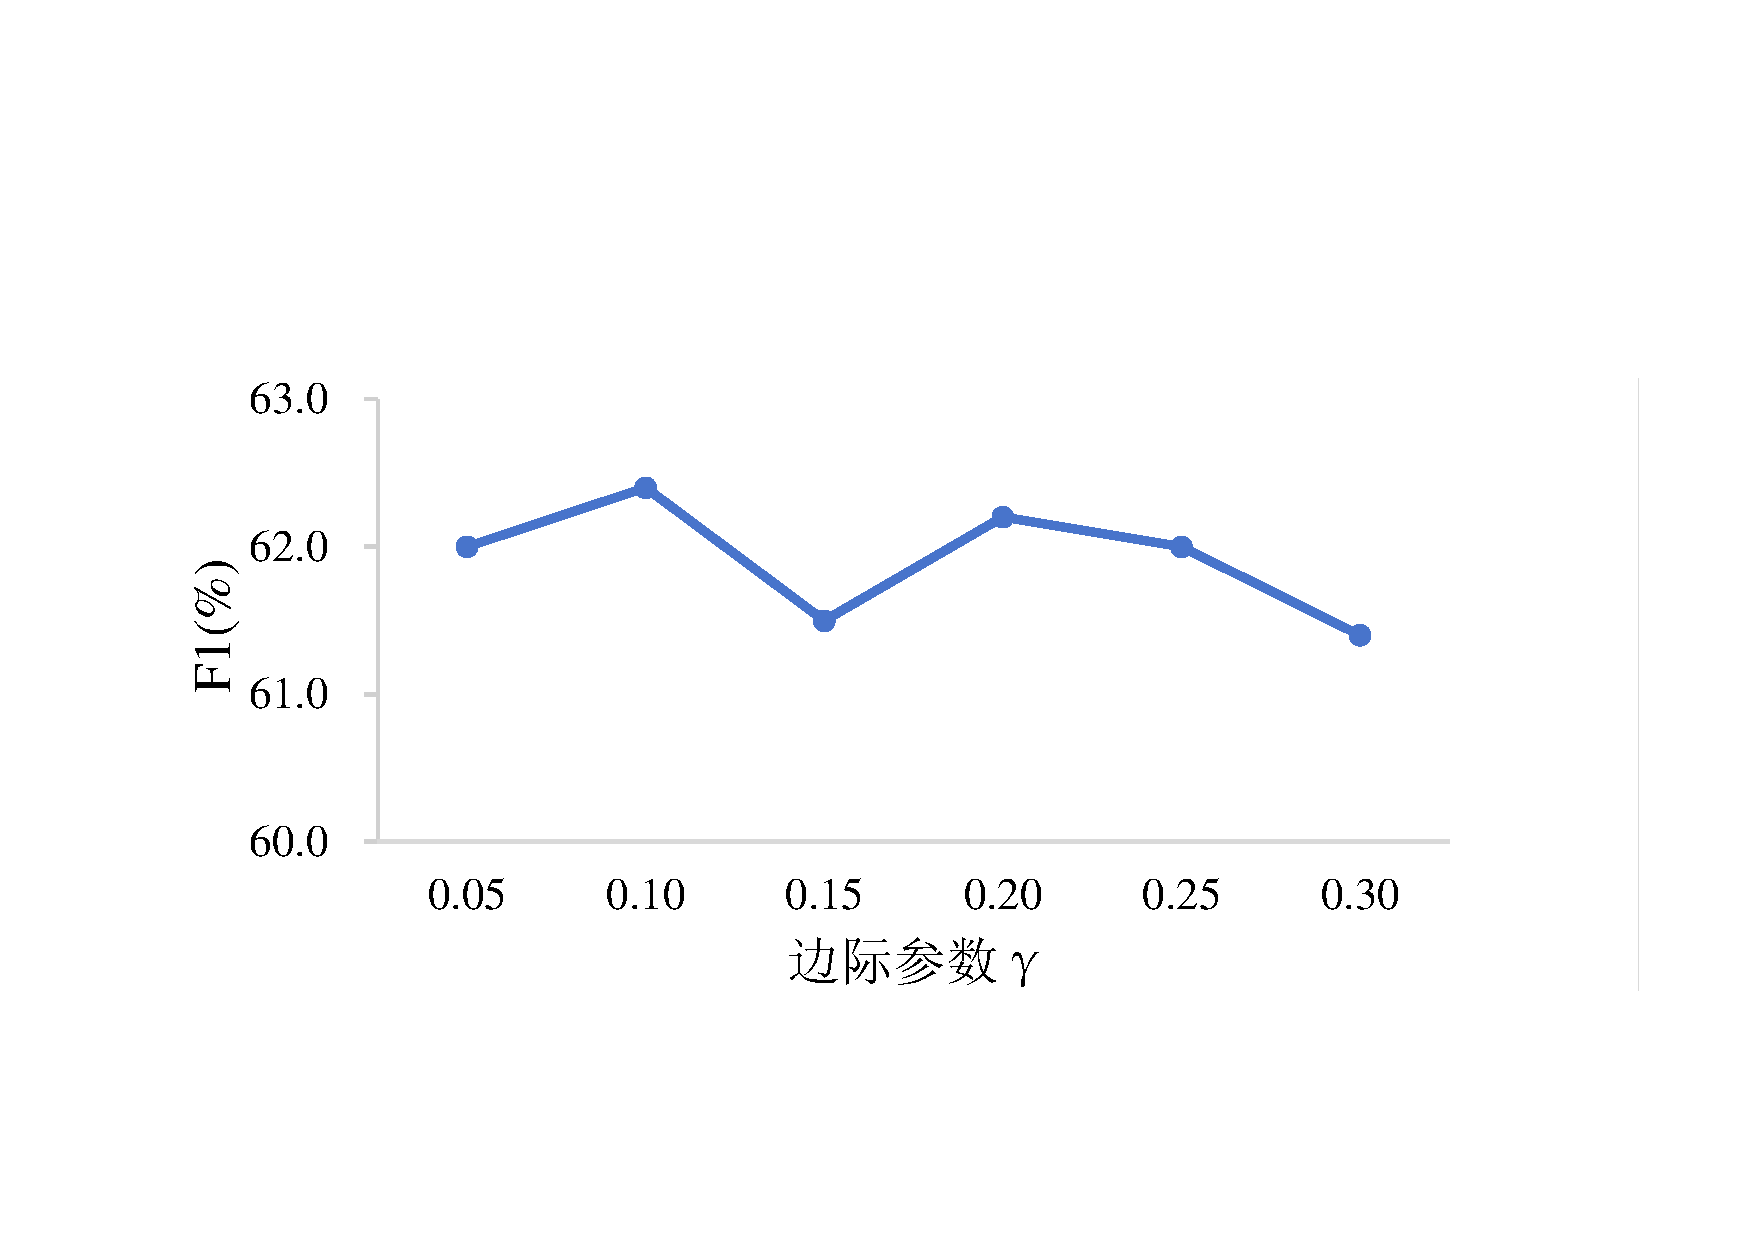
\includegraphics[width=0.6\linewidth]{figures/chap4/margin.pdf}
\label{margin}
}
\quad
\subfigure[]{
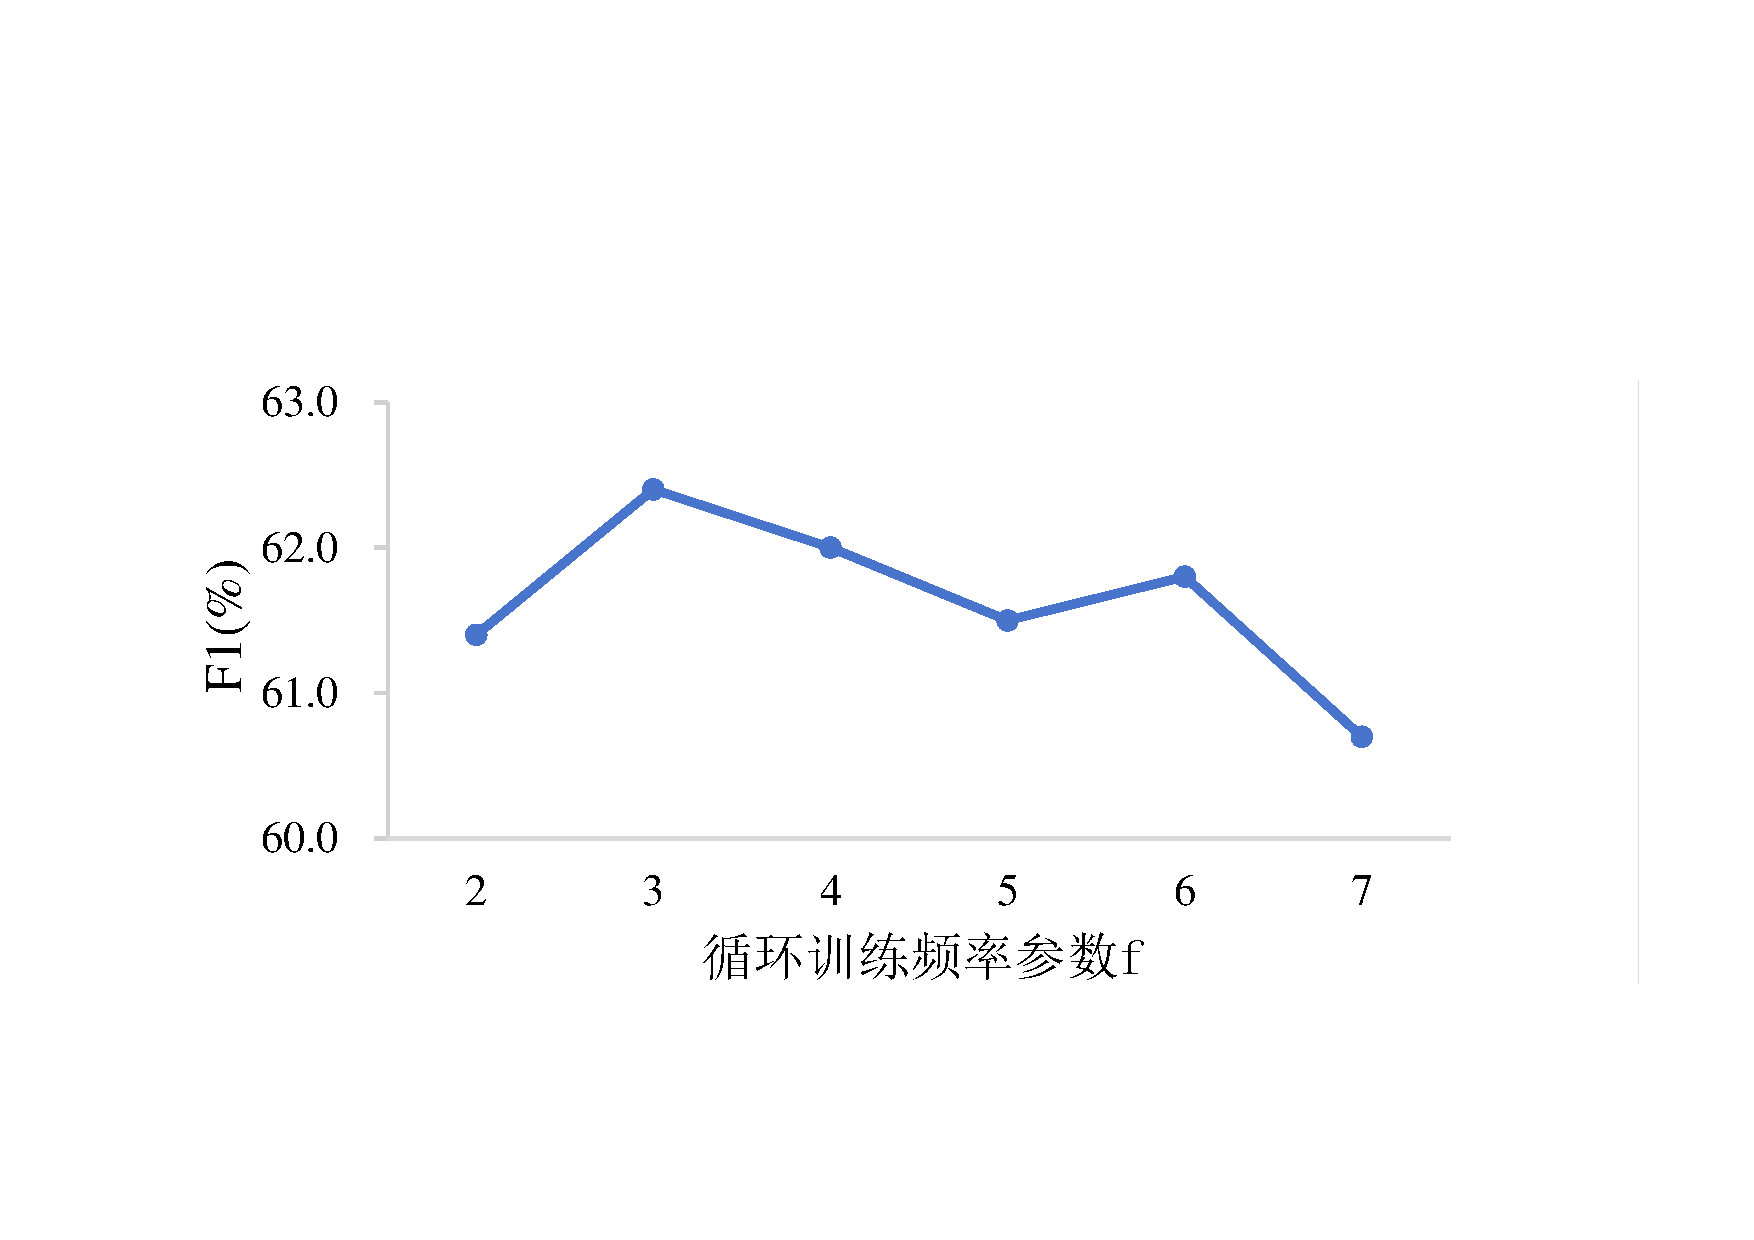
\includegraphics[width=0.6\linewidth]{figures/chap4/frequency.pdf}
\label{frequency}
}
\caption{METOR模型参数敏感性分析}
\label{sensitivity}
\end{figure*}

\subsection{计算复杂度分析}
虽然本章所提方法在实验中应用到了不同的事件要素抽取模型,但计算复杂度的分析是相似的。因此,本节着重讨论基于DMBERT的METOR模型的情况,具体计算如下:在编码器模块中,BERT的计算复杂度主要来源于多头注意力~\cite{vaswani2017attention},为$O~(N^2 d+Nd^2)$,其中$N$是输入序列的最大长度,$d$是BERT隐藏层输出向量的维度。在正样本处理模块中,语义相关性信息的计算复杂度为$O~((d_{s}^2 +d_{s})n_{e})$,其中$d_{s}$是事件类型/实体类型/要素类型向量的维度,$n_{e}$是给定事件要素抽取数据集中预定义实体类型的数目。对于基于NT-Xent的对比学习来说,其计算复杂度为$O~((d+d_{s}+d_{2})d_{1}+K d_{2}+K^{2})$,其中$d_{1}$和$d_{2}$是维度参数,$K$是批数据大小。在负样本处理模块中,计算复杂度为$O~(d_{2})$。在循环训练策略模块中,多类分类器的计算复杂度为$O~(n_{r}(d+d_{s}))$,其中$n_{r}$是给定事件要素抽取数据集中预定义要素类型的数目。

因此,METOR模型的总计算复杂度为$O~(N d^{2}+(N^{2}+d_{1}+n_{r})d+(d_{1}+K)d_{2}+n_{e}d_{s}^2+(d_{1}+n_{r}+n_{e})d_{s}+K^2)$。如果忽略较小的参数$n_{e}$, $n_{r}$和$d_{s}$,则其计算复杂度可以简化为$O~(N d^{2}+(N^{2}+d_{1})d+(d_{1}+K)d_{2}+K^2)$。进一步,与计算复杂度为$O~(N d^{2}+N^{2}d)$的基线模型DMBERT相比,所提模型的计算复杂度增长了$O~(d_{1} d+(d_{1}+K) d_{2}+K^2)$。由于在本章的超参数设置中,存在$d_{1}+K<d$,$d_{2}<d$和$K < N$,使得增长的计算复杂度$O~(d_{1} d+(d_{1}+K) d_{2}+K^2)$约等于$O~(d^{2}+N^{2})$。因此,可以得知METOR模型的计算复杂度略高于DMBERT,但其F1性能显著提高了5.2\%。

\subsection{案例研究}
本章节选取ACE2005数据集测试集中的六个实例进行案例研究。表\ref{case}展示了使用DMBERT、DMBERT(CL)和本章所提的METOR模型对这些实例的预测结果,其中DMBERT(CL)为表\ref{analysis}中的变体模型DMBERT+type+CL。

\begin{table*}[htp]
\footnotesize
\centering
% \setlength{\abovecaptionskip}{0pt}
% \setlength{\belowcaptionskip}{10pt}
\caption{ACE2005数据集上的案例分析}
% The trigger words and event argument candidates are in red and blue, respectively.}
\begin{tabular}{lcccc}
\toprule
\multicolumn{1}{c}{实例}    & 实体类型  & DMBERT & DMBERT (CL)  & METOR \\ \midrule
\begin{tabular}[c]{@{}l@{}}(1) Liana Owen drove 10 hours from \\ Pennsylvania to attend the \textcolor{red}{rally} in \\ \textcolor{blue}{Manhattan} with her parents.\end{tabular}              & County-or-District & Place $\checkmark$     &  Place $\checkmark$   & Place $\checkmark$     \\ \midrule
\begin{tabular}[c]{@{}l@{}}(2) He asked \textcolor{blue}{the court} to invalidate \\ the \textcolor{red}{verdict} and throw out the criminal \\ case against Pasko.\end{tabular} & Government & Adjudicator $\checkmark$ & Adjudicator $\checkmark$ & Adjudicator $\checkmark$ \\ \midrule
\begin{tabular}[c]{@{}l@{}}(3) Separately, \textcolor{blue}{former WorldCom} \\ \textcolor{blue}{CEO Bernard Ebbers} failed on April \\ 29 to make a first repayment of 25 \\ million dollars on a 400-million-dollar \\ \textcolor{red}{loan} from MCI, the Journal said, citing\\ SEC documents.\end{tabular}    & Individual  & Giver $\times$      & Recipient $\checkmark$ & Recipient $\checkmark$      \\ \midrule
\begin{tabular}[c]{@{}l@{}}(4) U.S. Defense Secretary Donald H. \\ Rumsfeld discussed the resolution with \\ Prime Minister Tony Blair and Defense \\ Secretary Geoff Hoon on Friday as \\ Rumsfeld \textcolor{red}{returned} from a tour of Iraq, \\ \textcolor{blue}{Afghanistan} and the Persian Gulf region.\end{tabular}                                    & Nation & Destination $\times$    &  Origin $\checkmark$   & Origin $\checkmark$    \\ \midrule
\begin{tabular}[c]{@{}l@{}}(5) It was not clear \textcolor{blue}{how many people} \\ were in the cafe at the time of the \textcolor{red}{blast}.\end{tabular}                                    & Indeterminate      & None $\times$    &  None $\times$   & Target $\checkmark$    \\ \midrule
\begin{tabular}[c]{@{}l@{}}(6) The space agency has been under \\ intense scrutiny since February when \\  \textcolor{blue}{the space shuttle Columbia} disintegrated \\ over Texas,  \textcolor{red}{killing} all seven crew \\ members.\end{tabular}  & Air     &  Instrument $\times$    &  Instrument $\times$   & None $\checkmark$    \\ \bottomrule
\end{tabular}
\label{case}
\end{table*}

在实例(1)中,“rally”触发了$Demonstrate$事件,且事件候选要素为“Manhattan”,其实体类型和要素类型分别为$County-or-District$和$Place$。由于实体类型$County-or-District$通常以要素类型$Place$参与到事件中,为该要素类型预测提供了重要信息。因此,DMBERT、DMBERT(CL)和本章所提的METOR模型通过实体类型$County-or-District$提供的语义信息给出了正确的要素类型预测。

在实例(2)中,候选事件要素“the court”的实体类型和要素类型分别为$Government$和$Adjudicator$。虽然实体类型$Government$无法提供明显的语义信息来预测要素类型,但当“verdict”触发的$Convict$事件给出时,其可以为预测提供信息提示。换而言之,$Government$实体经常在$Convict$事件中以要素类型$Adjudicator$出现,所以三个模型均能正确预测要素类型。因此,前两个实例证明了实体类型可以为预测其频繁参与的要素类型提供有用的预测线索。

在实例(3)中,在由“loan”触发的$Transfer-Money$事件中,候选事件要素“former WorldCom CEO Bernard Ebbers”的实体类型和要素类型分别为$Individual$和$Recipient$。由于要素类型$Giver$和$Recipient$均与实体类型$Individual$在$Transfer-Money$事件中频繁关联,DMBERT无法在该实例中正确区分$Giver$和$Recipient$。然而,DMBERT(CL)和本章所提的METOR模型均受益于对比学习,避免被同一事件中具有相同实体类型的要素类型所混淆,给出了正确的识别结果。实例(4)展示了另一个类似的实例。

在实例(5)中,候选事件要素“how many people”的实体类型和要素类型分别为$Indeterminate$和$Target$。从语义上来看,如果候选要素为一个$Indeterminate$实体,则该实体很有可能在事件中不作为要素出现。这种强语义关联导致了DMBERT对要素类型的预测错误。进一步,由于多数实体类型为$Indeterminate$的候选要素在训练集中不为
事件要素出现,DMBERT(CL)使用传统的对比学习来避免对于实体类型$Indeterminate$过度依赖的效果不佳。然而,本章所提的METOR模型消解了这种实体类型过度依赖问题,避免了该错误。

在实例(6)中,在由“killing”触发的$Die$事件中,候选事件要素“the space shuttle Columbia”的实体类型和要素类型分别是$Air$和$None$。和实例(5)相似,如果候选事件要素为一个$Air$实体,则该实体很有可能在事件中以要素类型$Instrument$出现,这阻碍了DMBERT和DMBERT(CL)从文本中理解语义信息,导致它们做出错误的预测。与之相比,METOR模型正确预测了要素类型。因此,METOR可以同时减少假负(false negative)预测(如实例(5)所示)和假正(false positive)预测(如实例(6)所示),从而取得优秀的事件要素抽取性能表现。

\section{本章小结}
本章首先研究了事件要素抽取的实体类型依赖性,并利用预实验评估其对不同事件要素抽取基线模型整体性能的影响。预实验表明了不同基线模型均面临不同程度的实体类型过度依赖问题,从而降低了整体性能。为此,本章提出了基于多角度对比学习的实体类型过度依赖消解方法。该方法分别从正样本和负样本角度消解模型在训练过程中对于实体类型的过度依赖,并设计了一种循环训练策略使这两种对比学习方法能够高效协作。本章基于ACE2005数据集进行了充分的实验,结果表明所提方法能够有效地对不同事件要素抽取基线模型进行实体类型过度依赖问题的消解,且当应用在DMBERT基线时,性能显著优于当前最佳的事件要素抽取模型。